\documentclass[12pt,a4paper]{report}
\usepackage{geometry}
\geometry{hmargin=2.5cm,vmargin=1.5cm}
\usepackage[utf8]{inputenc}
\usepackage[francais]{babel}
\usepackage[T1]{fontenc}
\usepackage{amsmath}
\usepackage{amsfonts}
\usepackage{amssymb}
\usepackage{graphicx}
\usepackage{lmodern}
\usepackage{xcolor}
\usepackage{cover}
\usepackage{fancyhdr}
\usepackage[final]{pdfpages}


\pagestyle{fancy}
\lhead{Pierrick CHOVELON - Julien TIRON}
\rhead{INF 112}

%%%% debut macro %%%%
\makeatletter
\renewcommand{\fnum@figure}{\small\textbf{\figurename~\thefigure}}
\renewcommand{\fnum@table}{\small\textbf{\tablename~\thetable}}
\makeatother
%%%% fin macro %%%%


\renewcommand{\familydefault}{\sfdefault} 
%\renewcommand{\scdefault}{\sfdefault} 

\definecolor{VertClair}{cmyk}{0.4,0.1,1,0}
%\definecolor{VertClair}{RGB}{168,181,10}
\definecolor{VertFonce}{cmyk}{1,0.55,0.5,0.5}
% \makeatletter
% \renewcommand\section{\@startsection {section}{1}{\z@}%
%                                    {-3.5ex \@plus -1ex \@minus -.2ex}%
%                                    {2.3ex \@plus.2ex}%
%                                    {\normalfont\Large\bfseries\color{VertClair}}}
%\parskip=3pt

\renewcommand{\chaptername}{} %les chapitres auront pour texte "Partie"

\begin{document}

\frontcover{
    Binôme :\\
    Pierrick CHOVELON\\
    Julien TIRON\\
    \vspace{1cm}
    FIP 1A}
  {Rapport Projet ToutAvis\\[10pt] INF112}
  {Formation d'ingénieur par partenariat
  \vspace{1cm}}
  {Version : 1\\ 
  \vspace{1cm}
  26 mai 2015}

\newpage
\tableofcontents
\newpage

\chapter*{Introduction}
\label{chapter:Introduction} %Ajout dans la table des matières
\addcontentsline{toc}{chapter}{Introduction}
\indent Ce rapport a pour but de dresser un bilan le plus complet possible du projet mené en INF112. Vous trouverez dans ce rapport les différentes informations concernants le projet ToutAvis et le travail que nous avons fourni pour le mener à bien. Vous trouverez dans chaque section quelques explications permettant de mieux comprendre notre démarche.

\chapter*{Fiche tâches/temps}
\label{chapter:Fiche tâches/temps} %Ajout dans la table des matières
\addcontentsline{toc}{chapter}{Fiches tâches/temps}


\chapter*{Diagramme de classes et diagrammes de séquences}
\label{chapter:Diagramme de classes et diagrammes de séquences} %Ajout dans la table des matières
\addcontentsline{toc}{chapter}{Diagramme de classes et diagrammes de séquences}
Vous trouverez dans les pages suivantes, les 3 diagrammes qui nous ont été demandés. \\

Nous avons essayé de faire un diagramme de classe le plus simple possible pour facilité la compréhension de la structure du projet pour des personnes extérieur à celui-ci.

Le diagramme de séquence de reviewOpinion (Fig. \ref{fig:diagSeq1}) peut sembler trop simple. Nous avons choisi de ne représenter que le cas de fonctionnement normal (i.e les données passées en paramêtres sont valides). 

\begin{figure}[h]
\centering
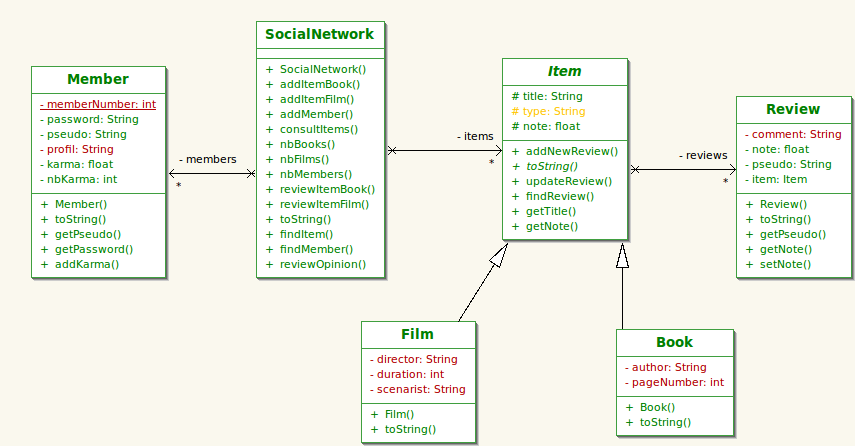
\includegraphics[angle = 90, scale=0.85]{Classe1.png}
\caption{Diagramme général de classes}
\label{fig:diagClasses1}
\end{figure}

\begin{figure}[h]
\centering
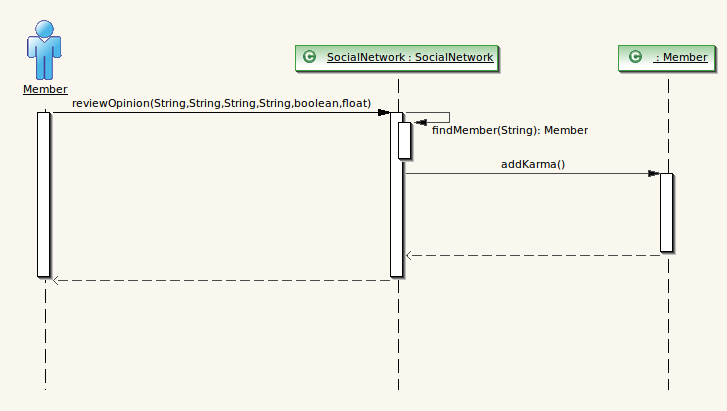
\includegraphics[angle = 90, scale=0.85]{Sequence1.png}
\caption{Diagramme de séquence de reviewOpinion}
\label{fig:diagSeq1}
\end{figure}


\begin{figure}[h]
\centering
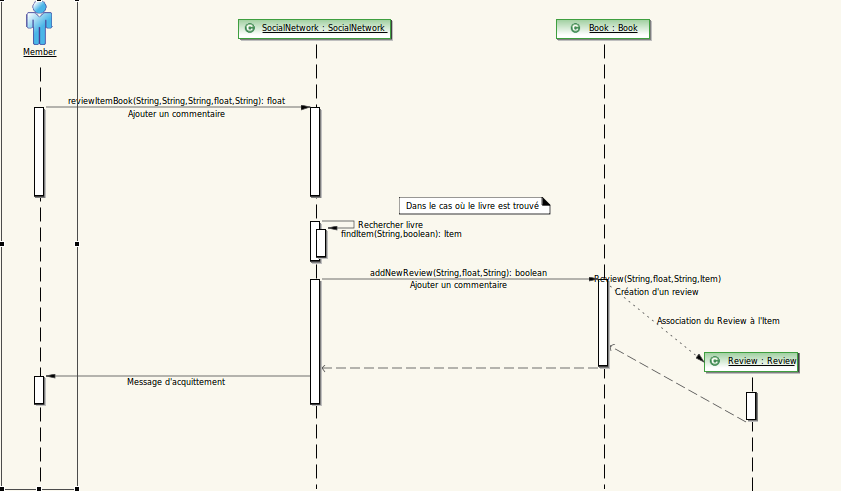
\includegraphics[angle = 90, scale=0.85]{Sequence2.png}
\caption{Diagramme de séquence de reviewItemBook}
\label{fig:diagSeq2}
\end{figure}

\chapter*{Rapport d'audit}
\label{chapter:Rapport d'audit} %Ajout dans la table des matières
\addcontentsline{toc}{chapter}{Rapport d'audit}
Le rapport d'audit effectué par un autre binôme nous a amené à changer notre code. Au total, se sont 8 remarques qui nous ont été faites. 7 d'entre elles concernaient un problème de fond et 1 un problème de forme. Nous avons acceptés 7 remarques. La remarque que nous avons refusée ne nous semblait pas opportune (gravité mineure). \\

La remarque de forme était très pertinente. En effet, le problème remonté était que nous utilisions toujours les mêmes conditions pour tester la validité des paramêtres donnés (\emph{pseudo}, \emph{password}, etc). Le copier-coller, rendant la tâche facile, nous à permis de réutiliser les condions des blocs \emph{if} aisément. Cependant, il est plus ingénieux et réfléchis de créer des fonctions qui renvoient \emph{true} ou \emph{false} selon un paramêtre donné. Ainsi, s'il faut modifier la manière dont est testé le \emph{password} par exemple, il suffit de modifier la fonction. Toutes les conditions utilisant cette fonction seront donc à jour, contrairement à la méthode que nous avions utilisée.\\

Les autres remarques, bien que pertinentes, n'étaient pas rès grave et relevait la plupart du temps d'un manque d'explication dans les commentaires.

\chapter*{Rapport de recette}
\label{chapter:Rapport de recette} %Ajout dans la table des matières
\addcontentsline{toc}{chapter}{Rapport de recette}
Lors de cette recette, aucune erreur n'a été relevée par le binôme client. Aucune modification n'a donc été apportée. Le fait que nos tests, ainsi que les tests du binôme client, ne relèvent aucune erreur nous permet donc de s'assurer de la conformité de notre livrable par rapport au cahier des charges.

\chapter*{Bilan}
\label{chapter:Bilan} %Ajout dans la table des matières
\addcontentsline{toc}{chapter}{Bilan}


\chapter*{Bilan général}
\label{chapter:Bilan général} %Ajout dans la table des matières
\addcontentsline{toc}{chapter}{Bilan général}
Pour dresser un bilan général du travail réalisé, nous pouvons tout d'abord dire que nous avons réussi à s'organiser au sein du binôme pour se répartir au mieu les tâches. De plus, l'utilisation de solution de <<versioning>> à grandement facilité le partage et la mise en commun du code.
\begin{quotation}
\textit{• Quels sont les points faibles et les points forts de votre livrable ?}
\end{quotation}

Le livrable que nous proposons est, d'une part, simple à comprendre grâce à la javadoc et, d'autre part, fidèle au cahier des charges grâce notamment à la batterie de tests effectués sur celui-ci. En plus des tests <<classiques>> sur les méthodes et les classes qui vont être utilisées, nous avons effectués des tests de rendement sur l'utisalisation de celle-ci. 

\begin{quotation}
\textit{• Si c'était à refaire, que changerions-nous, le cas échéant, dans notre démarche de conception-réalisation ?}
\end{quotation}

Pour reprendre la remarque relevée lors du rapport d'audit, nous pouvons dire qu'une des erreurs que nous avons faite a été de commencer le codage des méthodes trop rapidement. En soit, le premier code proposé n'était pas mauvais, mais il n'était pas correctement structuré. En effet, un temps de réflexion au préalable, sur les fonctions et les conditions qui allaient être appelées fréquement, nous aurait permis de gagner du temps en fin de projet. 

\begin{quotation}
\textit{• Quels sont les avantages et inconvénients trouvés dans la démarche de conception en W ?}
\end{quotation}


\chapter*{Annexes}
\label{chapter:Annexes} %Ajout dans la table des matières
\addcontentsline{toc}{chapter}{Annexes}



\end{document}